\documentclass[a5paper,fontsize=10pt]{memoir}
\usepackage[
  top=2cm,bottom=2cm,
  inner=1.75cm,
  outer=1.25cm,
  textwidth=13cm
]{geometry}
\strictpagecheck

\usepackage[utf8]{inputenc}
\usepackage[german]{babel}

\usepackage{palatino}
\usepackage[T1]{fontenc}

\usepackage{graphicx}
\usepackage{hyperref}
\usepackage{hyphenat}
\usepackage{fancyhdr}
\usepackage{pdfpages}

\renewcommand{\headrulewidth}{0pt}
\pagestyle{fancyplain} % Makes all pages in the document conform to the custom headers and footers
\fancyhead[L]{}% Empty left header
\fancyhead[C]{\thepage} % Page numbering for center header
\fancyhead[R]{}% Empty right header
\fancyfoot[L]{}% Empty left footer
\fancyfoot[C]{}% Empty center footer
\fancyfoot[R]{}% Empty left footer

\begin{document}
\pagenumbering{gobble}

{\centering
{\Large Vorwort}
\vspace{2em}

\begin{minipage}{4cm}
  \hrulefill\\
\end{minipage}

}
\vfill
Abraham Gerardus van Stipriaan Luïsçius%
\footnote{\href{https://web.archive.org/web/20210927050342/https://www.geni.com/people/Abraham-van-Stipriaan-Luïscius/6000000011599769478}
{geni.com/people/Abraham-van-Stipriaan-Luïscius/6000000011599769478}}
konnte am 10. August 1798
seinen nachfolgend behandelten Artikel in der holländischen Zeitung
\emph{Nieuwe allgemeene Konst - en Letter Bode}
abdrucken lassen.
Dieser wurde ein Jahr später
von Dr. August Friedrich Adrian Diel%
\footnote{\href{https://web.archive.org/web/20160828042236/https://de.wikipedia.org/wiki/Adrian_Diel}
{de.wikipedia.org/wiki/Adrian\textunderscore Diel}}
ins Deutsche übersetzt und unter dem Titel
\emph{Art und Weise,
um das laugensalzige Luftsauerwasser
(\texttt{aqua mephitica alcalina})
mit leichter Mühe, und ohne Kosten
vermittelst des Fachinger Mineralwassers zuzubereiten}%
\footnote{\href{https://archive.org/details/b30350360}
{archive.org/details/b30350360}}
dem deutschsprachigen Raum in broschierter Form
zur Verfügung gestellt.

Im Folgenden habe ich erwähnte Schrift
in eine leichter lesbare Form übertragen --
dabei Grammatik beibehalten,
Orthografie nach persönlichem Ermessen angepasst
und erweiterte Fußnoten eingesetzt,
um z.B. verwendete Einheiten in metrische Maße umzurechnen
oder, soweit wie möglich, modernere Terminologie anzubieten.

Abgesehen von der Namensverwandschaft
ist die Motivation und das Pflichtgefühl dahinter
die Hoffnung,
ähnlich der von A. v. Stipriaan Luïsçius,
dass sich mehr ``Landsleute'' informieren und ein
mit wesentlichen 
%nicht-organischen Salzen (Spurenelementen)
angereichertes Wasser
in die alltägliche Anwendung bringen können.
Beim Lesen habe ich ein einprägsames Gefühl für den Wert
eines solchen Wassers bekommen,
auch durch den speziellen Charakter der damaligen Zeit.

Falls der Leser
stellenweise an alten Formulierungsarten
oder recht wissenschaftlichen Inhalten anecken
sollte, ermutige ich diesen,
solche Stellen zu überfliegen und dort fortzusetzen,
wo wieder mehr Lesefluss möglich ist.
Die Thematik ist heute mindestens so aktuell, wie damals.
Die praktische Anwendung 
ist heutzutage glücklicherweise um einiges einfacher,
welche ich im Anhang näher beschreibe.

\pagenumbering{Roman}
\setcounter{page}{1}

Nachfolgend an die Transkription folgen:
\begin{itemize}
\item Herleitung der korrekten Maßumrechnungen
\item Analyse der Vorgehensweise von A. v. Stipriaan Luïsçius
\item Anmerkungen und Vergleiche
zum heutzutage käuflichen sog. ``Staatl. Fachingen Wassers'',
um eine Perspektive aufzuzeigen,
warum es dennoch sinnvoll sein kann,
ein solches Wasser selber herzustellen oder
alternative Angebote von Elektrolyt-Wasser zum Kauf anzubieten
\item zeitgemäße Wege und Ansätze, ein qualitativ hochwertiges Wasser selber herzustellen
\end{itemize}

Es war eine kleine Reise,
erst das Dokument zu lesen,
ohne im ersten Anlauf den Inhalt im Detail verstanden zu haben --
aber wohl erkennen konnte,
dass hier ein kleiner Schatz verborgen liegt;
dann das Dokument abzutippen
und in eine neues Format zu übertragen,
dabei ins tiefere Verständnis zu kommen,
etwas über Chemie, Physiologie und Geschichte zu lernen;
dann im Detail zu analysieren, umzurechnen,
den Aufbau und die Chemie,
alles nach bestem Wissen und Gewissen nachzuvollziehen
\emph{und} -- ganz am Ende -- den tatsächlichen Schatz zu heben.
Denn als ich das Beschriebene begriff,
war der ``Zauber'' kurz vorbei
und dachte: \emph{wie einfach!}
Und mit Hinblick auf moderne und alternative Forschungen
konnte ich weitere Zusammenhänge dahingehend herstellen,
wie bedeutend das Ganze selbst für unsere heutige Zeit ist,
darauf hoffend, dass sich mehr Menschen
solches Wissen zu Eigen machen wollen.

Die Fußnoten des Originaldokumentes
sind in kleinen römischen Zahlen ausgezeichnet,
wobei meine eigenen Fußnoten lateinisch nummeriert sind.
Alle hierin angegebenen Internet-Quellen
sind auch auf archive.org gesichert und wiederzufinden. 

Dieses Buch ist auf Github%
\footnote{\href{https://github.com/gogolnr1/aqua-mephitica-alcalina}{github.com/gogolnr1/aqua-mephitica-alcalina}}
unter der Creative Commons Lizenz%
\footnote{CC BY-NC-SA (\href{https://creativecommons.org/licenses/by-nc-sa/3.0/de/}{creativecommons.org/licenses/by-nc-sa/3.0/de/})},
inklusive des Originaldokumentes von Dr. Friedrich Diel,
zu finden.
Letzteres wird in diesem Jahr genau 222 Jahre alt.
%
\fancyhead{}
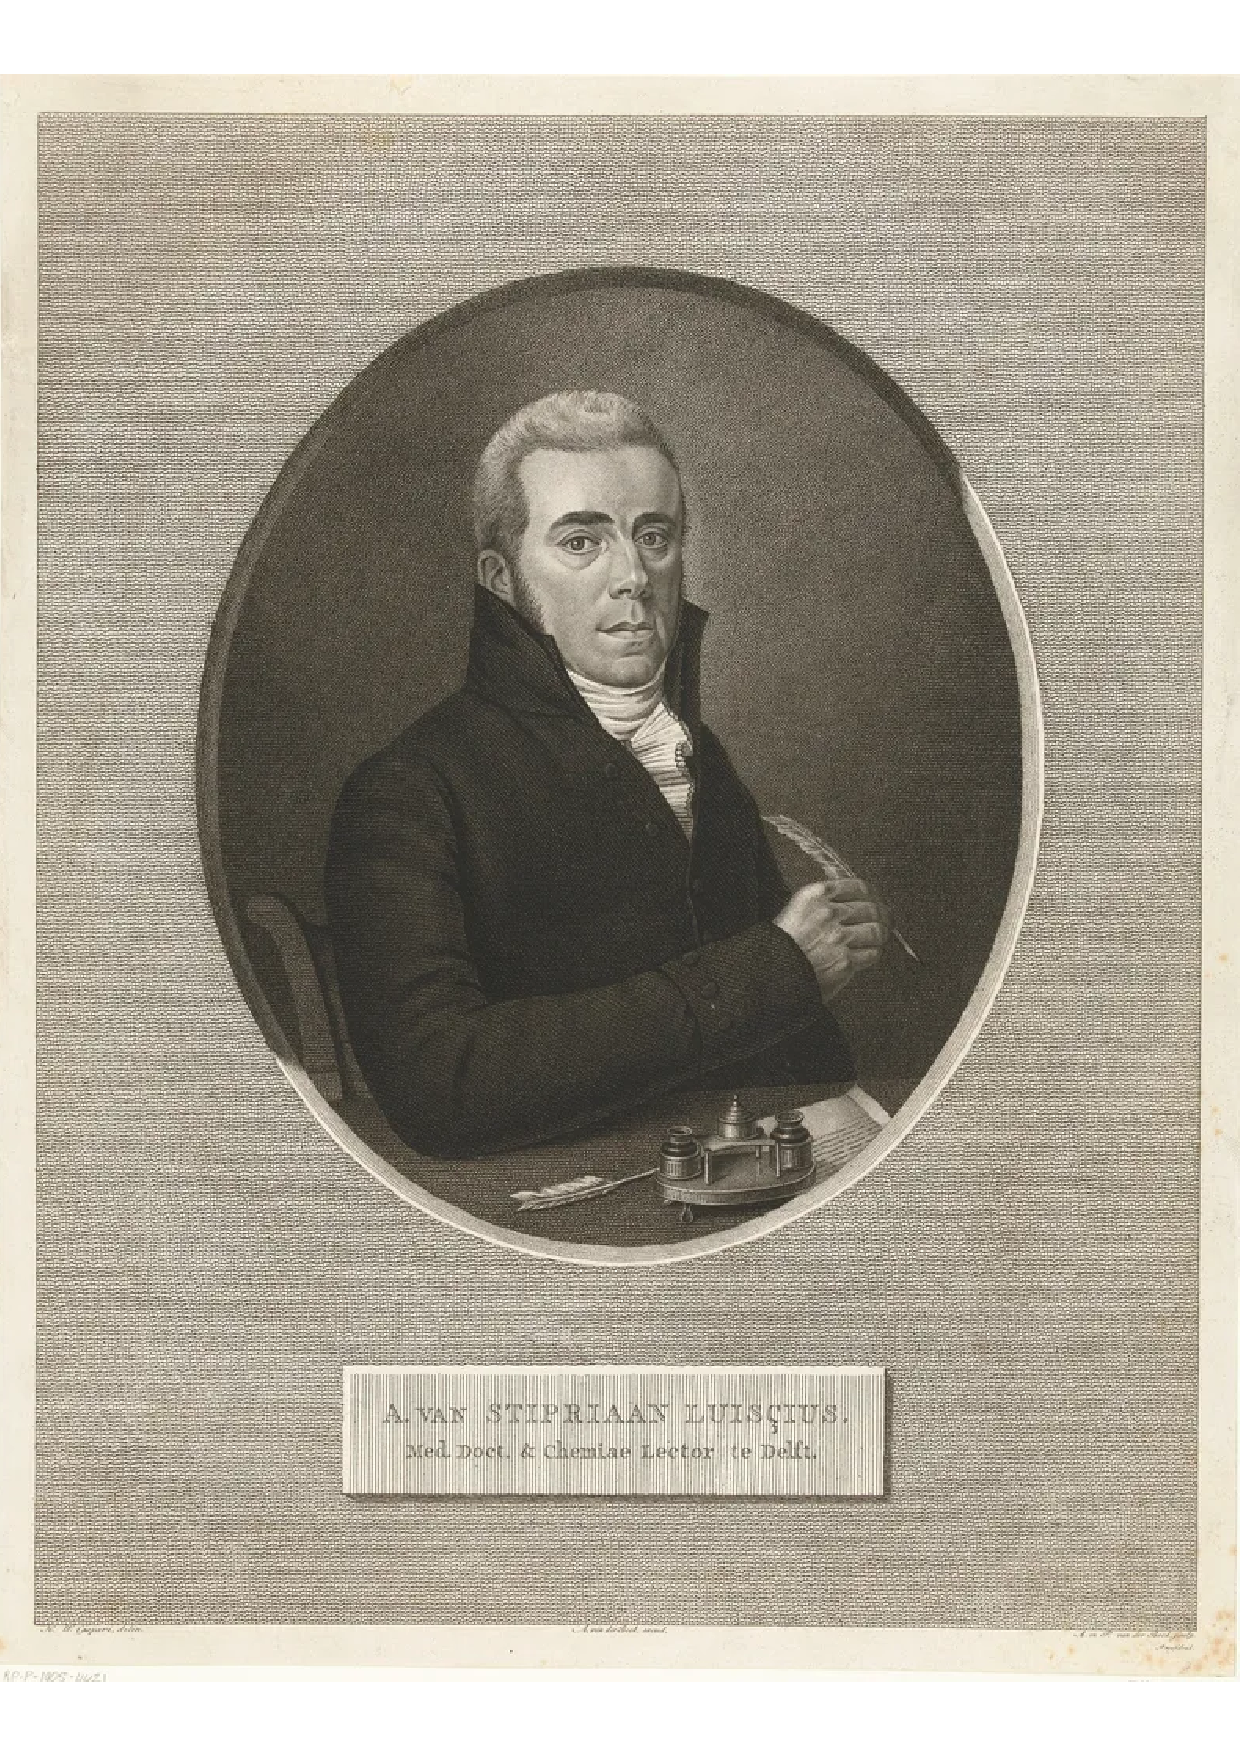
\includepdf{../figures/portrait.pdf}\strut%
%
% if pagenumber uneven, make newpage
\checkoddpage\ifoddpage%
  \newpage\strut%
  \fi

\end{document}
